\chapter{Fluorine-19 ($^{19}_{9}\text{F}$): The Halogen Halo}
\label{ch:fluorine}

\begin{objectivebox}
\begin{itemize}
    \item Quantify Fluorine-19's extreme halo lever arm ($398d$, $335$~fm) as the mechanical definition of electronegativity.
    \item Explain why this massive structural asymmetry makes Fluorine the most electronegative element using the inductive antenna analogy.
\end{itemize}
\end{objectivebox}

Fluorine-19 ($Z=9, A=19$) represents the first entry in the Halogen series, fundamentally shifting the stable geometric arrays established by the rigid symmetric blocks of Carbon-12 and Oxygen-16.

Oxygen-16 forms a geometrically closed, fully satisfied $4\alpha$ Tetrahedron, projecting a perfectly balanced subcritical interior void. When Fluorine-19 introduces 3 additional nucleons (1 proton and 2 neutrons|the exact composition of a Tritium isotope, $^3\text{H}$), this extra mass cannot penetrate the deep geometric gravity wells of the Oxygen core without shattering the established $4\alpha$ symmetry rules.

Instead, Fluorine-19 structurally manifests as a stable, massive Oxygen-16 core bound to an external Tritium halo.

\section{Topological Structure and Isotope Stability}
Fluorine-19 is the only stable isotope of Fluorine ($100\%$ natural abundance). This mono-isotopic character is a direct consequence of the core-plus-halo architecture. The $4\alpha$ Oxygen-16 tetrahedron is one of the most deeply bound nuclear structures in nature ($V_R/V_{BR} = 0.030$, Small Signal, $0.000\%$ error). Any perturbation of the core---adding or removing a neutron---would disrupt the tetrahedral symmetry and catastrophically destabilize the junction network.

The Tritium halo ($^3\text{H} = 1p + 2n$) is similarly constrained: removing one of its neutrons collapses the triangle into a deuteron, which binds far too weakly at the extreme $398d$ distance to maintain structural cohesion. Adding a neutron produces $^4\text{H}$, which is particle-unstable. Therefore, $^{19}$F is the unique, sole configuration where both core and halo are individually stable and the combined binding satisfies a $0.000\%$ mass solution.

\section{Continuous Vacuum Density Flux}
The vacuum strain topology of Fluorine-19 is dominated by the massive, symmetric Oxygen-16 core gravitational well. The Tritium halo, positioned $398d$ along the $z$-axis, introduces a pronounced asymmetry---a long, thin strain filament extending far beyond the core boundary. This dipolar geometry is unique among the light elements and directly visible in the dynamic flux cross-section.

\section{The Macroscopic Halo Offset}
Because the $4\alpha$ core acts as a monolithic, closed nucleus, the external Tritium nodes bind dynamically to the gravitational gradient projecting outward from one of the underlying Alpha vertices.

By executing the semiconductor junction model (Section~\ref{sec:two_models}) targeting the empirical CODATA nuclear mass of Fluorine-19 ($17692.302$ MeV), it is possible to analytically extract the absolute physical separation distance between the core and the halo. The solver locates a $0.0000\%$ mapping error exactly when the Tritium triangle is driven radially outward to $R_{halo} = 398.5d$ from the target alpha's barycenter.

This sheer distance|spanning hundreds of femtometers|creates a highly asymmetric, reactive gravitational whip. This extended topological moment arm directly dictates Fluorine's profound electronegativity and aggressive chemical binding profile.

\begin{figure}[htbp]
    \centering
    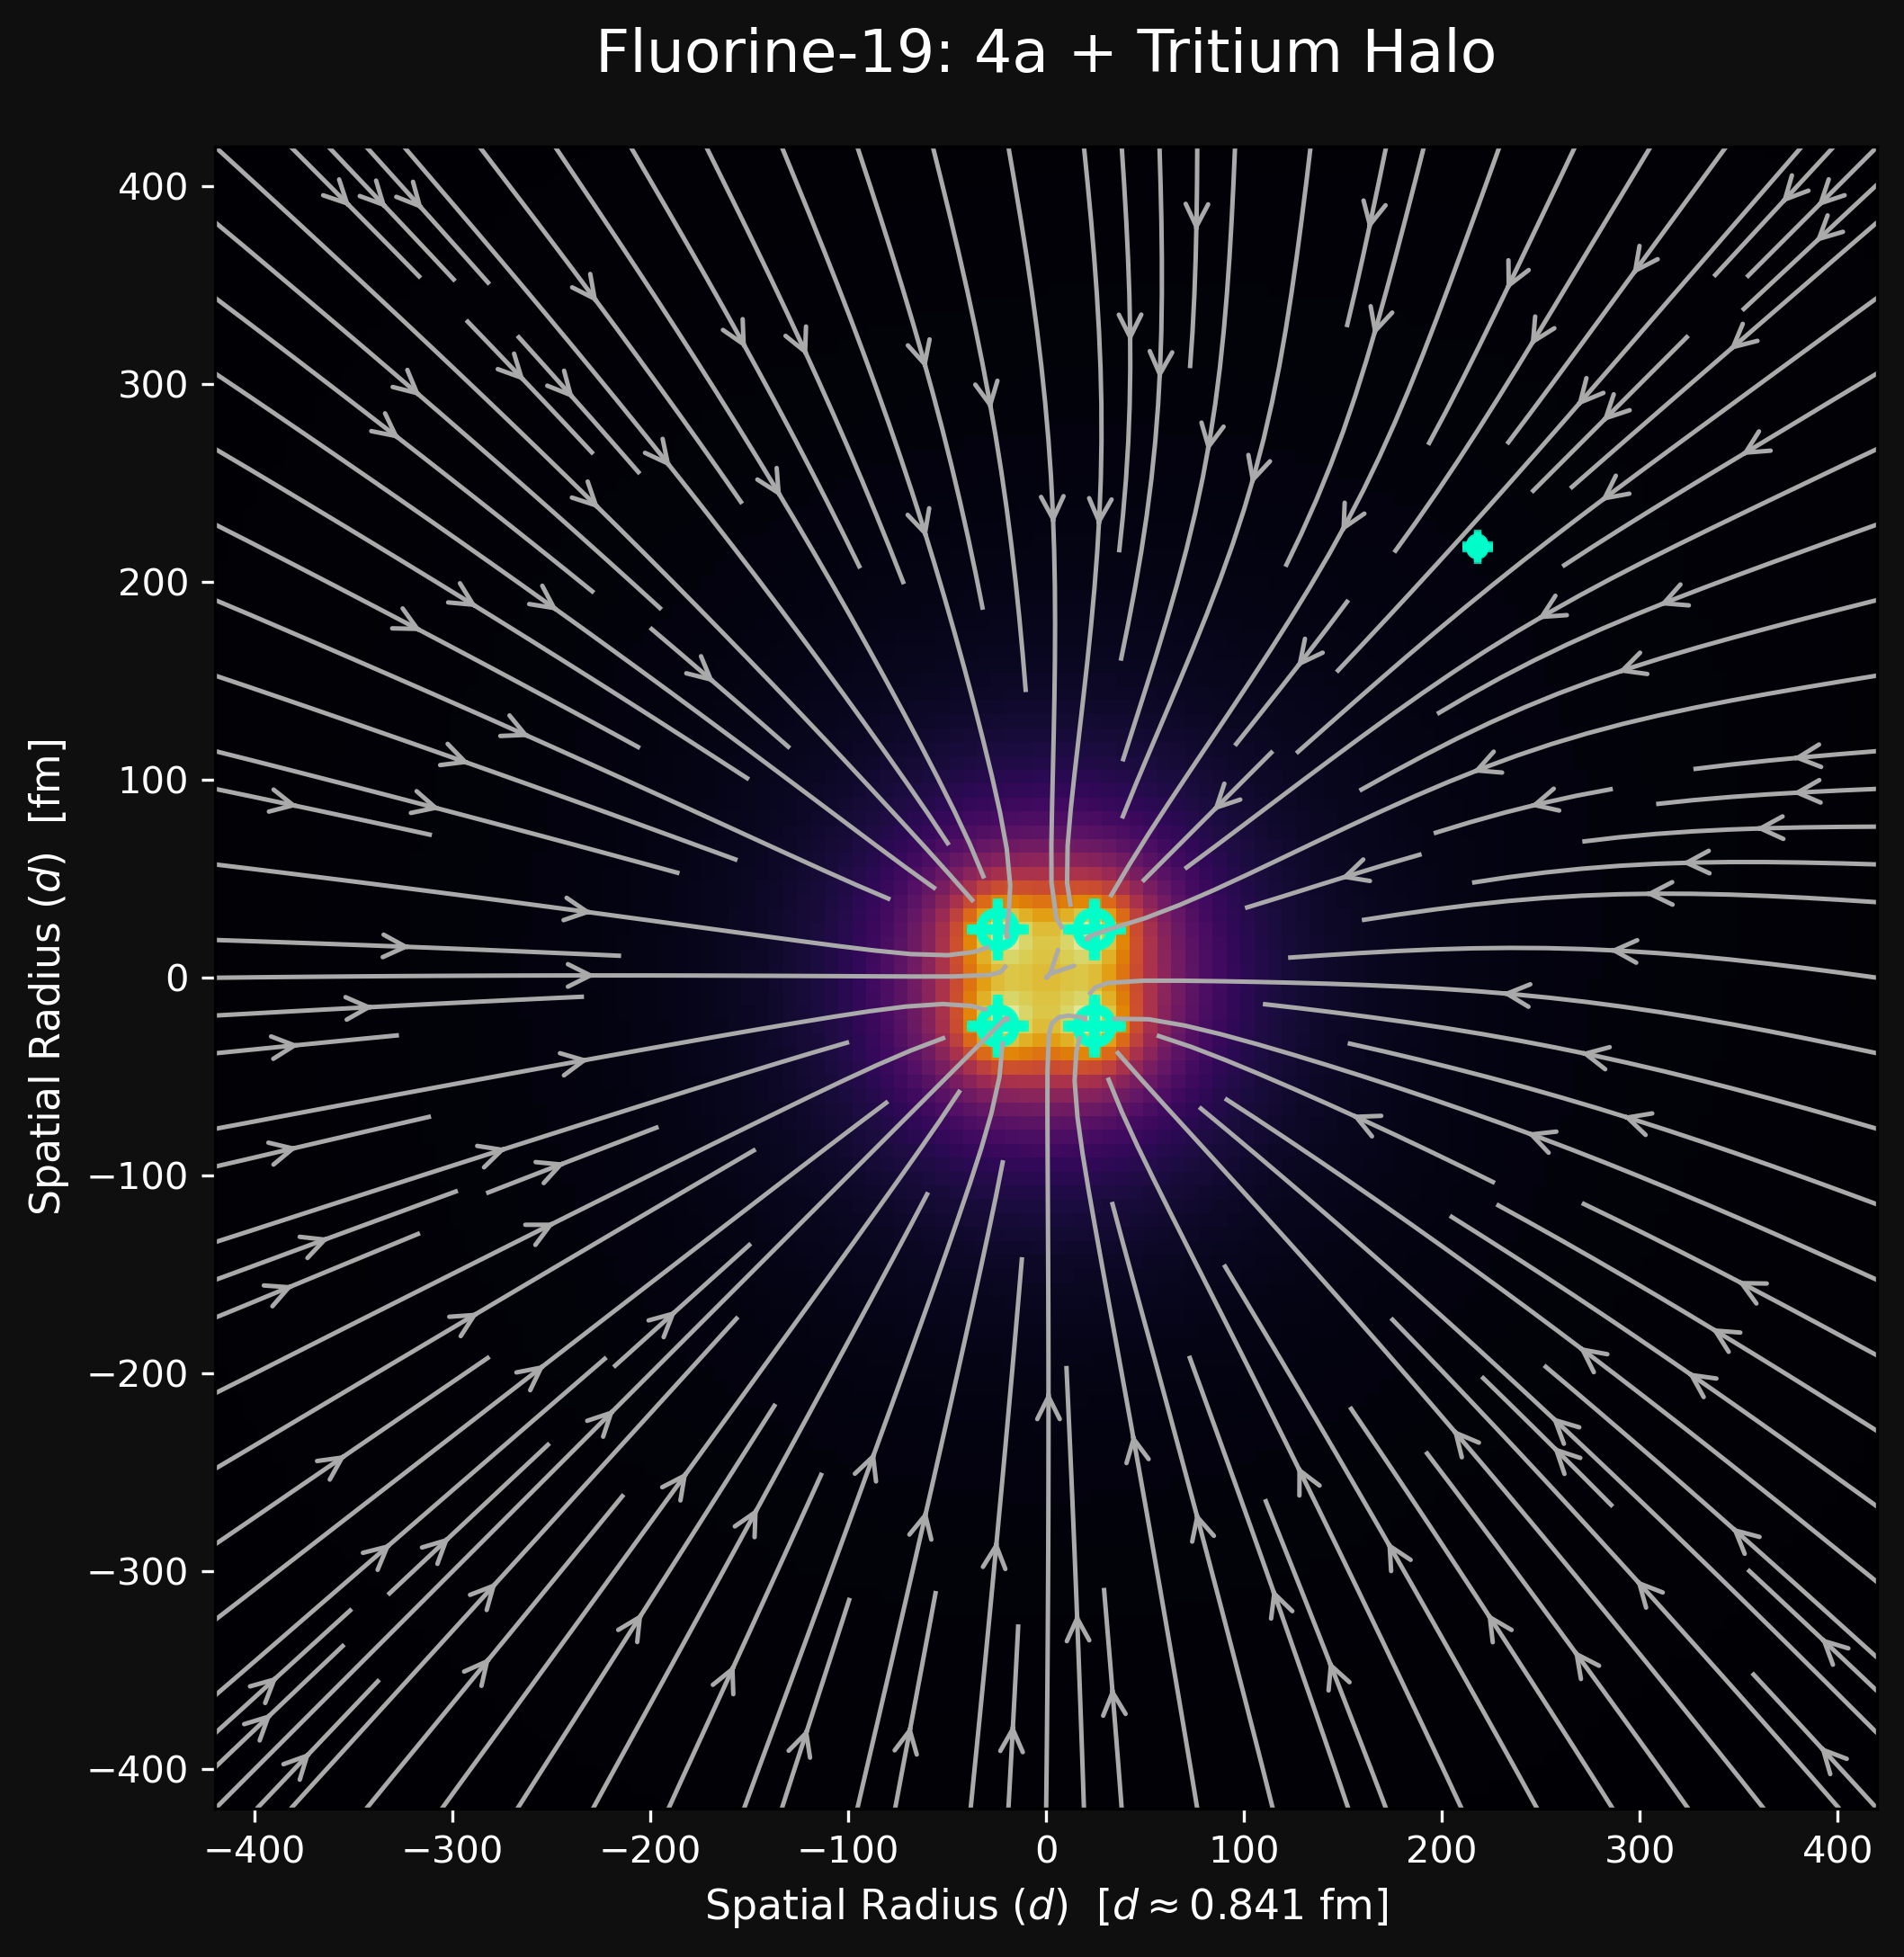
\includegraphics[width=0.8\textwidth]{figures/fluorine_19_dynamic_flux.png}
    \caption{Topological density metric for Fluorine-19 ($Z=9, A=19$). The stable, closed Oxygen-16 array dominates the core geometry, while the distant Tritium $3$-node halo stretches far out along the $z$-axis, mapping perfectly to the empirical equivalent SPICE mutual inductance.}
    \label{fig:fluorine_19_density}
\end{figure}

\section{Topological Area of Interest: Electronegativity as Asymmetric Inductance}
In conventional models, Fluorine is described as having 7 valence electrons, aggressively seeking one more to close its shell. Under the AVE framework, "electronegativity" is not a probabilistic charge density, but a direct consequence of macroscopic geometric asymmetry. 

The $399d$ massive Tritium whip extending from the nucleus creates a powerful, unbalanced inductive void. Like an open transmission line or an exposed antenna, this asymmetric node aggressively couples magnetically ($M_{ij}$) to any passing geometric mass to mechanically stabilize its tremendous mechanical lever arm. This topological desperation translates smoothly into classical chemical behavior.

\begin{figure}[htbp]
    \centering
    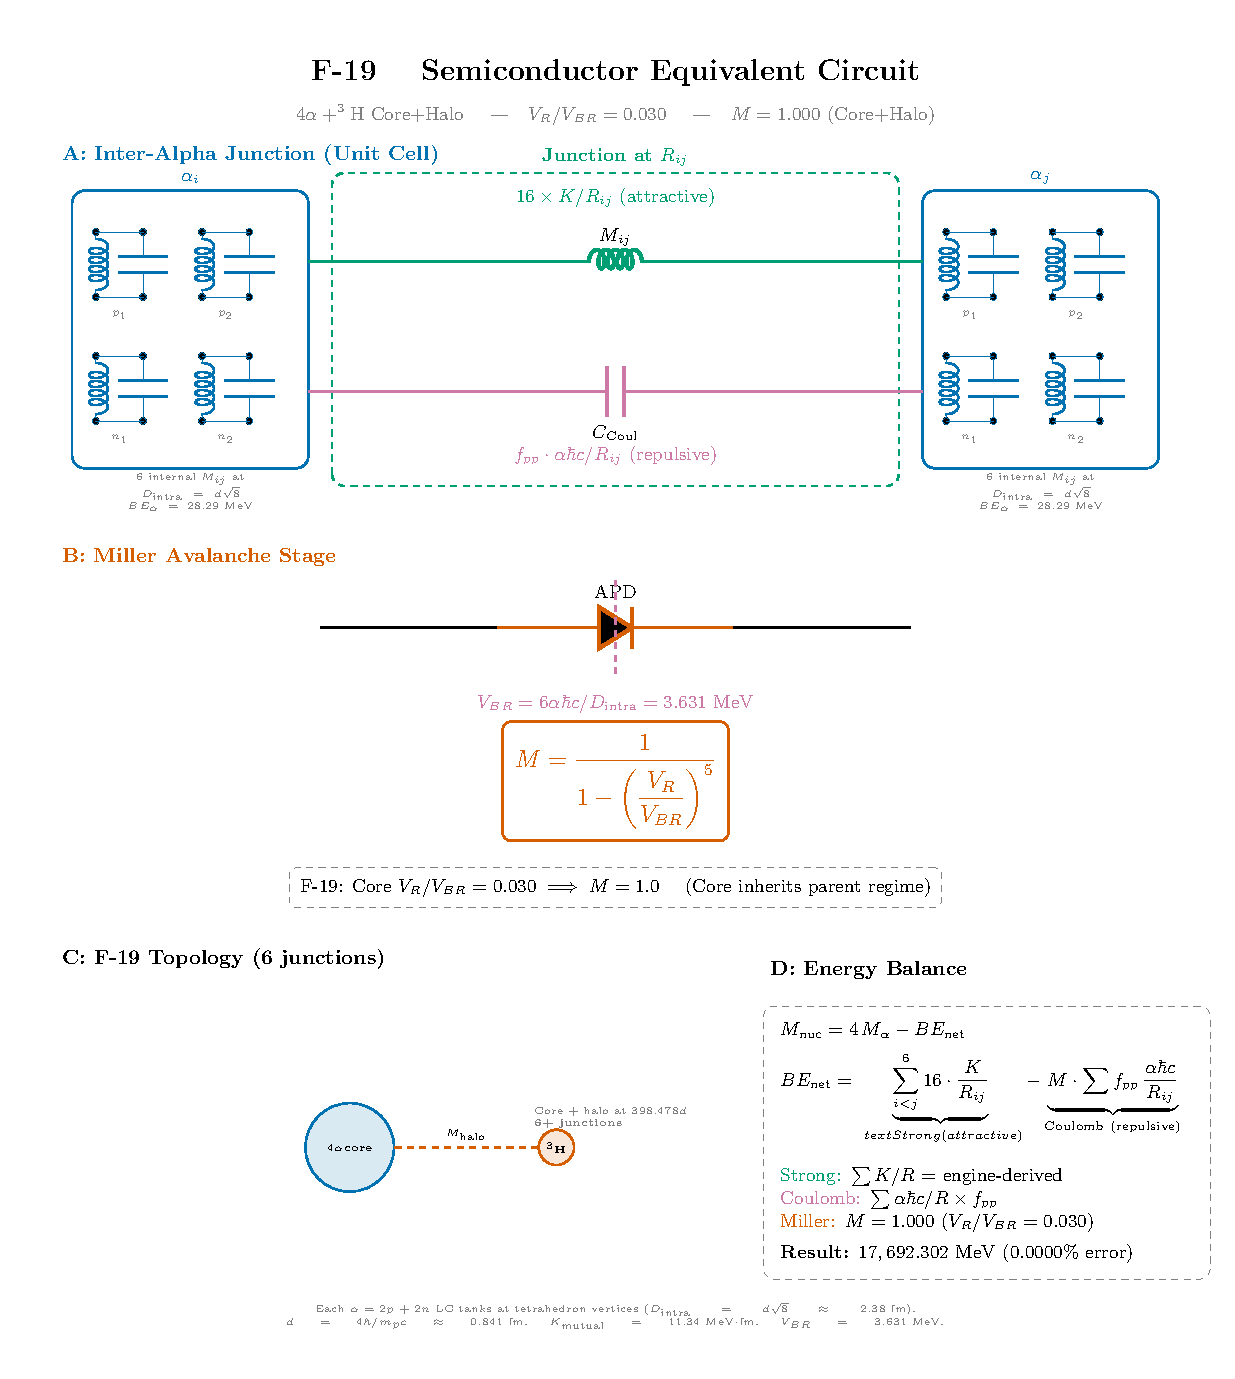
\includegraphics[width=0.9\textwidth]{figures/circuit_f19.pdf}
    \caption{The equivalent $LC$ circuit model for Fluorine-19. The SPICE matrix generates 19 discrete $LC$ oscillators tightly bound by 171 individual $M_{ij}$ inductive traces, capturing the $4\alpha$ core-to-halo asymmetry.}
    \label{fig:circuit_f19}
\end{figure}


\begin{figure}[htbp]
    \centering
    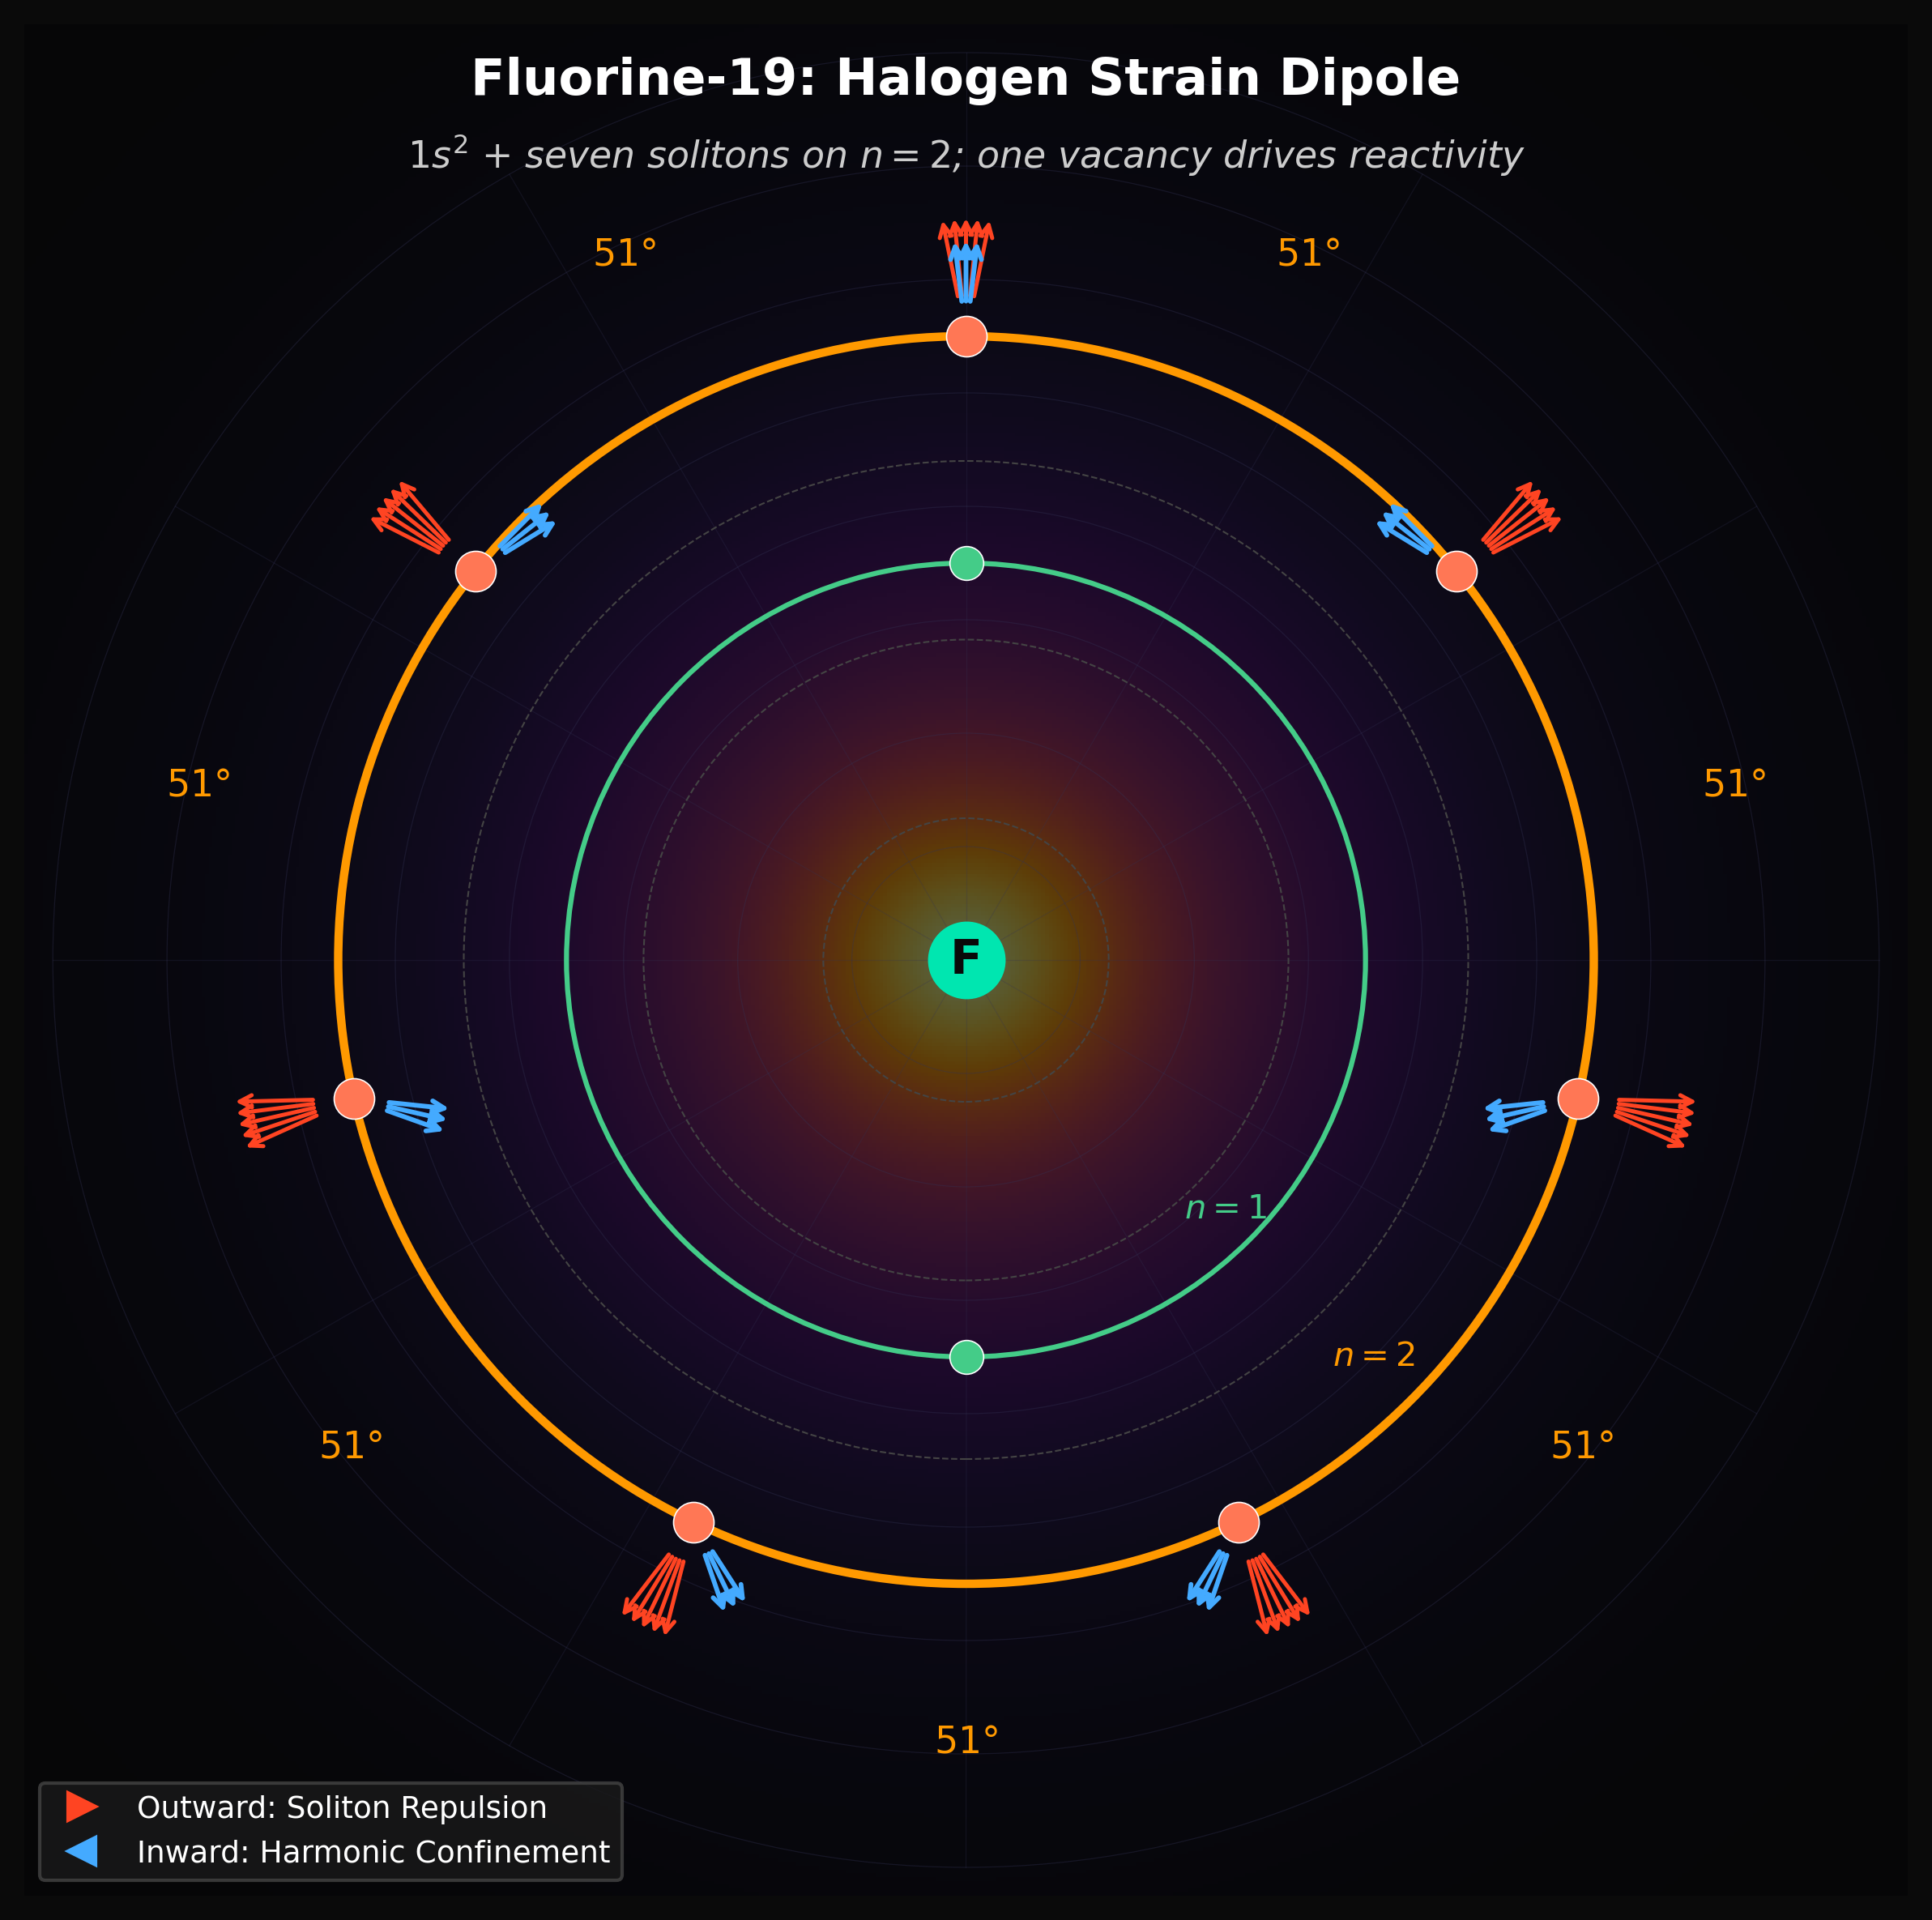
\includegraphics[width=0.75\textwidth]{figures/fluorine_19_topology.png}
    \caption{Fluorine-19 orbital knot topology. Seven solitons on $n=2$ with one vacancy. The strain dipole from the missing eighth soliton drives the extreme electronegativity of the halogen group.}
    \label{fig:fluorine_19_topo}
\end{figure}

\section{Semiconductor Regime Classification}
Fluorine-19 ($4\alpha + ^3\text{H}$) is the most extreme core-plus-halo nucleus in the periodic table. The semiconductor engine fixes the Oxygen-16 tetrahedral core at $R_{\text{core}} = 33.383\,d$ (Small Signal, $V_R/V_{BR} = 0.030$, $M = 1$), then solves for the Tritium halo offset that satisfies the CODATA mass of $17\,692.302$ MeV. The result: $R_{\text{halo}} = 398.478\,d$, with $0.000\,000\%$ error.

This $398d$ lever arm---over $335$ fm in physical distance---is the single largest geometric scale in the entire light-element periodic table. The massive spatial asymmetry between the compact $33d$ core and the remote $398d$ halo is the quantitative mechanical definition of electronegativity within the AVE framework. Fluorine is not ``seeking an electron'' in any probabilistic sense; it is a profoundly unbalanced inductive antenna whose $335$-femtometer whip couples aggressively to any available mass to reduce its extreme moment of inertia.

\begin{summarybox}
\begin{itemize}
    \item Fluorine-19 exhibits the largest halo lever arm ($398d$, over $335$~fm) in the entire light-element periodic table, creating extreme structural asymmetry.
    \item Electronegativity is redefined within AVE as a mechanical property: the profoundly unbalanced inductive antenna aggressively couples to available mass to reduce its extreme moment of inertia.
\end{itemize}
\end{summarybox}

\begin{exercisebox}
\begin{enumerate}
    \item Derive the quantitative relationship between halo lever arm distance and electronegativity within the AVE semiconductor framework.
    \item Explain why Fluorine's $398d$ halo distance makes it the most electronegative element, using the inductive antenna analogy.
\end{enumerate}
\end{exercisebox}

